\chapter{Overlapping Reconstructions}
\label{ch:overlapping}

\section{Purpose}
\label{sec:overlapping-purpose}

Frazier et al. demonstrate that the sona of a given interrogation pulse is significantly longer than the pulse that generated it~\cite{nltr-wave-chaotic}. This stands to reason, given that the sona represents reflections of the initial pulse shifted in time by differing path lengths.

The reverse is also true: A time reversed sona will generate a reconstruction that is significantly shorter than it in time. This trait imposes a limitation on the ability of time reversal to transmit power, especially given that it is difficult to pack a large amount of energy into a short period of time. Time increase the amount of energy transmitted, we desire to send reconstructions more frequently than the length of the sona will allow. However, transmitting multiple sonas at once from the same antenna is possible--copying and shifting the signal in time can allow several signals to be sent in less time than the sum of the individual sona time lengths. This will in turn result in multiple transmitted reconstructions, and improved power transmission.

A concern with the above method is whether or not it would result in lost information and consequently degraded reconstruction quality. Sonas are sinusoidal signals--if overlaid, they will interfere constructively and destructively. Destructive interference may result in the ``deletion'' of transmission paths, reducing the efficiency of the TR process and decreasing the fidelity of the created reconstructions. In this experiment, we are interested in understanding the degree to which superimposing sonas will degrade the ability to transmit energy between ports using linear time reversal.

\section{Methodology}
\label{sec:overlapping-meth}

This test sought to evaluate the practicality of overlapping sonas as a method of transmitting power. This experiment was done using the basic, two-port linear time reversal scheme, described in Section~\ref{sec:linear-methodology}. A sona was generated with a 3.9 GHz interrogation pulse. To verify that the sona could converge on the target, it was time reversed without any further manipulation, and injected back into the cavity. The reconstruction was recorded and compared to the original interrogation pulse to check for irregularities.

Once the efficacy of the single sona was established, the experiment was modified. Several sonas were superimposed with a constant time shift, resulting in evenly spaced copies of the verified sona across the total broadcast window. Figure~\ref{fig:overlapping-sonas} gives an example of sonas overlapping in this way. The resulting signal was then time reversed and broadcast through the linear system in the same manner as before, which resulted in the reconstructions in Figure~\ref{fig:overlapping-recons}. This test was repeated many times, with time offsets varying between 0.1~$\mu$s and 15~$\mu$s, by increments of 0.1~$\mu$s.

\begin{figure}[t]
\centering
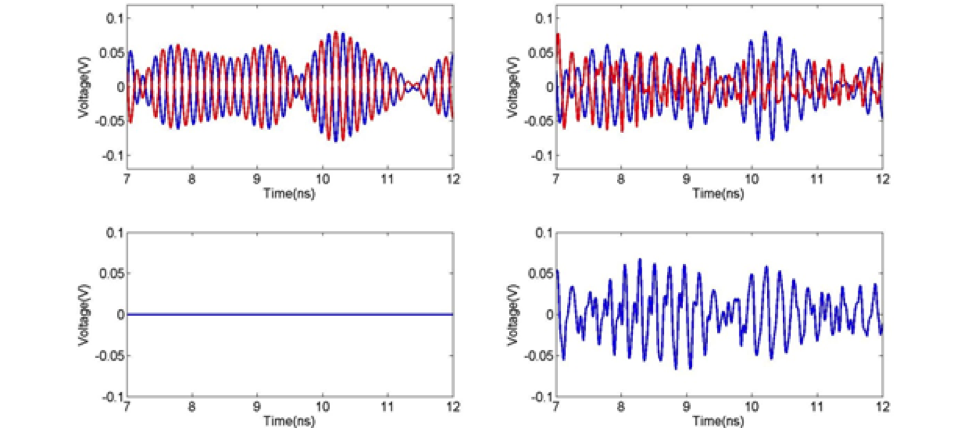
\includegraphics[width=0.85\textwidth]{overlapping/sonas}
\caption[Overlapping sonas]{Overlapping sonas with a spacing of 7.5 $\mu$s.}
\label{fig:overlapping-sonas}
\end{figure}

\begin{figure}[t]
\centering
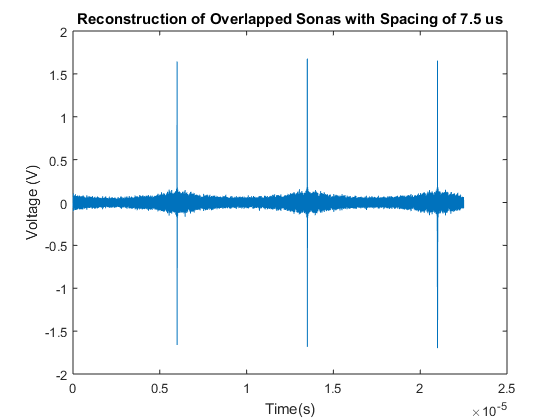
\includegraphics[width=0.85\textwidth]{overlapping/recons}
\caption[Overlapping reconstructions]{Reconstructions resulting from the sonas in~\ref{fig:overlapping-sonas}.}
\label{fig:overlapping-recons}
\end{figure}

\begin{figure}[t]
\centering
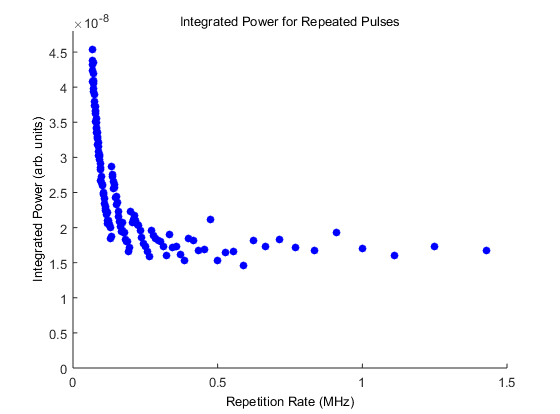
\includegraphics[width=0.85\textwidth]{overlapping/power}
\caption[Power from overlapping reconstructions]{Integrated power from overlapping reconstructions.}
\label{fig:overlapping-power}
\end{figure}

\section{Results}
\label{sec:overlapping-results}

For each setting of the time delay, a measure of the power received was calculated from a trapezoidal Riemann sum of the square of the recorded voltage across a recorded 15~$\mu$s window. We call this quantity the integrated power, and it is proportional to the power that is accepted at the receiver. The integrated power for each valoe of the repetition rate is plotted in Figure~\ref{fig:overlapping-power}. Increasing the number of sonas should increase the amount of power transmitted in a given time frame, if the amplitude of each reconstruction remains constant. However, we actually observed an inverse relationship between repetition rate of the sonas and total power within the recorded reconstruction signal. The trend observed in Figure~\ref{fig:overlapping-power} is more complex than we had anticipated, displaying stratified bands within an exponential decay envelope. 


\section{Discussion}
\label{sec:overlapping-discussion}

We hypothesized that overlapping reconsturctions by overlaying sonas could result in more effective power transmitted per duty cycle. Our experiments seemed to support this in that the number of reconstructions in the cycle could be increased while maintaining their characteristic shape. When the integrated power was plotted against the repetition rate, we found that the power actually exhibited the opposite trend as we had expected. We believe these results to be a combination of two factors. The loss of information due to destructive interference during sona superposition, and the function of power scaling within the PSG signal generator both may have contributed to these strange results. The generator attempts to level a preset amount of power across the entire broadcast window, which results in the discontinuities when mechanically switching source components throughout the sweep. However, without intimate knowledge of the PSG's inner workings, it is near impossible to extract any meaningful information regarding the origin of these bands. We recommend that future research be conducted on this phenomenon, to either confirm our results or to demonstrate that they are an artifact of our equipment limitations.
